\section{Fault Tolerance and Accountability}
\label{sec:ft}

By Property 1, one set of mechanisms must cover crashes, churn and malice. We now say how a failure is noticed, how a failed scheduler is replaced, and how work is accounted for.

\subsection{Progress, not liveness}
The hard failures are the ones where \emph{liveness signals look healthy}. A \emph{black-holing} host (a node that quietly swallows what it receives) keeps sending heartbeats while dropping the work it accepted. An on--off host builds a clean record and then defects. A drain notice may be a lie.
So we adopt a rule: \emph{liveness signals from untrusted machines are hints, and progress observed by trusted or attested parties is evidence.} The trusted observers are the routers. The attested observers are the worker agents and the scheduler code, although their \emph{hosts} are still untrusted for availability.

Each detector watches an event that must happen if a component works, and blames a suspect when it does not. The router's \emph{dispatch watchdog} suspects a scheduler when an enqueued invocation is not acknowledged within 1\,s.
The scheduler's \emph{result watchdog} suspects a worker that accepted work but has not returned a result by the predicted 90th-percentile completion time, times 1.2, and at least 3\,s. Repeated dispatch timeouts become a \emph{cluster-stall} report, and a \emph{decision-latency} limit on the scheduler's attested timestamps catches a scheduler that is alive but slow.
A running record of each worker's omission rate, with a change-point test, catches selective and on--off behaviour. Heartbeats stay as a fast path for plain crashes and are never sufficient alone.
A suspected worker gets no new work, its in-flight work is duplicated or retried, and it loses provisioned eligibility. A suspected scheduler triggers failover.

\subsection{Replacing a scheduler without consensus}
\label{sec:succession}
Once a failure is suspected, the scheduler must be replaced. The textbook way is a replicated state machine among the candidates, but that is slow, and it brings an agreement problem onto machines that may be adversarial.
\voss{} avoids the problem for two reasons: the provider's orchestrator is a reliable referee, and a scheduler's state is \emph{soft}. Figure~\ref{fig:failover} shows the sequence.

\textbf{Appointment and fencing.} The orchestrator appoints a scheduler by an atomic compare-and-swap on the cluster's \emph{epoch} number in its database, like a lease~\cite{burrows2006chubby}. The appointment binds the cluster, the epoch and the session-certificate identifier of the appointee, so a cloned appliance with a different session key is not appointed.
Workers accept dispatches only from the current epoch and certificate and answer older epochs with a \texttt{STALE} reply, which fences the old scheduler off. A scheduler that cannot reach the orchestrator for one lease period stops dispatching on its own.
A partitioned scheduler can therefore cause only duplicate work, which at-least-once execution allows. That is safe for idempotent functions. For a non-idempotent function, a duplicate sent within the lease period could repeat its effect, and the protocol does not prevent this (Section~\ref{sec:threats}).

\textbf{Soft state.} A scheduler keeps nothing durable on its host. Undispatched invocations are held by routers, running work and confirmed provisioning by workers, and estimator state in a checkpoint at the control plane.
After appointment the successor installs the new epoch and performs a \emph{roll call}: it asks the workers for their running work, confirmed pins and keys and recent outcomes, rebuilds its view and re-plans from the checkpoint. Because nothing authoritative lives on the old host, a restarted appliance is a new instance that must be appointed again.

\textbf{Succession.} The orchestrator keeps a ranked list of candidates by survival, speed, centrality and assurance, with diversity across failure domains. Every attested worker can serve, because the scheduler code is in the image, so promotion needs no boot. Planned handovers flush a checkpoint first, and a \emph{fake} drain by a malicious scheduler host just causes a clean handover.
With the broker of Section~\ref{sec:broker}, the successor takes over by subscribing to the cluster's scheduler topic.

\begin{figure}[t]
\centering
\resizebox{0.8\columnwidth}{!}{\begin{tikzpicture}[x=1mm,y=1mm]
  \def\seqh{104}
  \seqactor{7}{rt}{Router}
  \seqactor{28}{sc}{Sched.\\epoch 7}
  \seqactor{49}{or}{Orch.\\+ DB}
  \seqactor{70}{nx}{Succes-\\sor}
  \seqactor{88}{wk}{Workers}
  \seqmsg{-12}{rt}{sc}{ENQUEUE}{msg}
  \seqnote{28}{-18.5}{host crashes, or black-holes\\while heartbeats continue}
  \seqnote{7}{-27}{no ASSIGNED in $T_{\text{dispatch}}$:\\resend, spill sync}
  \seqmsg{-37}{rt}{or}{STALL(cluster, 7)}{msg}
  \seqnote{49}{-43.5}{CAS epoch $7\to8$; token\\binds successor's cert}
  \seqmsg{-51}{or}{nx}{APPOINT(8, checkpoint)}{msg}
  \seqmsg{-56}{or}{rt}{new scheduler, same topic}{rsp}
  \seqmsg{-63}{nx}{wk}{EPOCH\_INSTALL, ROLL\_CALL}{msg}
  \seqmsg{-69}{wk}{nx}{work, pins, keys, outcomes}{rsp}
  \seqnote{70}{-75.5}{rebuild view; replay outcomes;\\re-plan from checkpoint}
  \seqmsg{-83}{rt}{nx}{re-send pending (dedupe by id)}{msg}
  \seqmsg{-89}{nx}{wk}{DISPATCH(epoch 8)}{msg}
  \seqnote{88}{-96}{epoch $<8$: STALE}
\end{tikzpicture}
}
\caption{Scheduler failover. The router's dispatch watchdog detects a crashed or black-holing scheduler. The orchestrator changes the epoch atomically and appoints a successor, which rebuilds soft state from workers and a checkpoint.}
\label{fig:failover}
\end{figure}

\textbf{Worker failures.} When a session ends, keys and warm sandboxes vanish and the invocation is retried or duplicated elsewhere, preferring provisioned machines. A per-cluster retry budget and router spillover contain retry storms. Owner notices such as drain make the scheduler more careful but never excuse an omission in the estimators.

\subsection{Receipts and credits}
\label{sec:receipts}
Each result carries a receipt signed with the session key. It names the invocation and attempt, the worker and certificate, the epoch, the execution time, the work done in reference units and a digest of the output.
The router checks it against the certificate and the verifier's revocation list and appends it to the operational database. A machine cannot claim work it did not do. It can only decline to do work, which is an omission handled above.
Credits are proportional to reference work, not elapsed time, so throttling earns nothing, and a small credit rewards cache that the plan asked a host to hold. Reputation is kept apart from the survival and omission estimators, so no signal is counted twice, and it is used only for rewards and as a tie-breaker.
We leave out a blockchain on purpose. Receipts are already verifiable by third parties, and the only risk that remains is the control plane withholding records, which a signed transparency log would address better.
